
%(BEGIN_QUESTION)
% Copyright 2011, Tony R. Kuphaldt, released under the Creative Commons Attribution License (v 1.0)
% This means you may do almost anything with this work of mine, so long as you give me proper credit

The overhead pressure control system in this fractionator seems to have a problem.  The controller (PIC-33) indicates the pressure being over setpoint by a substantial margin: the pressure reads 48 PSI while the setpoint is 37 PSI:

$$\includegraphics[width=15.5cm]{i0001rx01.eps}$$

Identify the likelihood of each specified fault in this process.  Consider each fault one at a time (i.e. no coincidental faults), determining whether or not each fault could independently account for {\it all} measurements and symptoms in this process.

% No blank lines allowed between lines of an \halign structure!
% I use comments (%) instead, so that TeX doesn't choke.

$$\vbox{\offinterlineskip
\halign{\strut
\vrule \quad\hfil # \ \hfil & 
\vrule \quad\hfil # \ \hfil & 
\vrule \quad\hfil # \ \hfil \vrule \cr
\noalign{\hrule}
%
% First row
{\bf Fault} & {\bf Possible} & {\bf Impossible} \cr
%
\noalign{\hrule}
%
% Another row
PT-33 calibration error &  &  \cr
%
\noalign{\hrule}
%
% Another row
PY-33a calibration error &  &  \cr
%
\noalign{\hrule}
%
% Another row
PY-33b calibration error &  &  \cr
%
\noalign{\hrule}
%
% Another row
PV-33b block valve closed &  &  \cr
%
\noalign{\hrule}
%
% Another row
PV-33b bypass valve open &  &  \cr
%
\noalign{\hrule}
%
% Another row
Instrument air supply to PY-33b failed &  &  \cr
%
\noalign{\hrule}
%
% Another row
Instrument air supply to FV-34 failed &  &  \cr
%
\noalign{\hrule}
} % End of \halign 
}$$ % End of \vbox

\underbar{file i03533}
%(END_QUESTION)





%(BEGIN_ANSWER)

% No blank lines allowed between lines of an \halign structure!
% I use comments (%) instead, so that TeX doesn't choke.

$$\vbox{\offinterlineskip
\halign{\strut
\vrule \quad\hfil # \ \hfil & 
\vrule \quad\hfil # \ \hfil & 
\vrule \quad\hfil # \ \hfil \vrule \cr
\noalign{\hrule}
%
% First row
{\bf Fault} & {\bf Possible} & {\bf Impossible} \cr
%
\noalign{\hrule}
%
% Another row
PT-33 calibration error &  & $\surd$ \cr
%
\noalign{\hrule}
%
% Another row
PY-33a calibration error &  & $\surd$ \cr
%
\noalign{\hrule}
%
% Another row
PY-33b calibration error &  & $\surd$ \cr
%
\noalign{\hrule}
%
% Another row
PV-33b block valve closed & $\surd$ &  \cr
%
\noalign{\hrule}
%
% Another row
PV-33b bypass valve open &  & $\surd$ \cr
%
\noalign{\hrule}
%
% Another row
Instrument air supply to PY-33b failed &  & $\surd$ \cr
%
\noalign{\hrule}
%
% Another row
Instrument air supply to FV-34 failed &  & $\surd$ \cr
%
\noalign{\hrule}
} % End of \halign 
}$$ % End of \vbox

%(END_ANSWER)





%(BEGIN_NOTES)

Control strategy based on that shown on page 1179 of B\'ela Lipt\'ak's {\it Instrument Engineer's Handbook, Process Control}, Third Edition.  Embellishments added just to make the diagram more evil!

\vskip 20pt \vbox{\hrule \hbox{\strut \vrule{} {\bf Virtual Troubleshooting} \vrule} \hrule}

This question is a good candidate for a ``Virtual Troubleshooting'' exercise.  Presenting the diagram to students, you first imagine in your own mind a particular fault in the system.  Then, you present one or more symptoms of that fault (something noticeable by an operator or other user of the system).  Students then propose various diagnostic tests to perform on this system to identify the nature and location of the fault, as though they were technicians trying to troubleshoot the problem.  Your job is to tell them what the result(s) would be for each of the proposed diagnostic tests, documenting those results where all the students can see.

During and after the exercise, it is good to ask students follow-up questions such as:

\begin{itemize}
\item{} What does the result of the last diagnostic test tell you about the fault?
\item{} Suppose the results of the last diagnostic test were different.  What then would that result tell you about the fault?
\item{} Is the last diagnostic test the best one we could do?
\item{} What would be the ideal order of tests, to diagnose the problem in as few steps as possible?
\end{itemize}

%INDEX% Basics, control loop troubleshooting (realistic P&ID shown)
%INDEX% Process: distillation, generic (realistic P&ID shown)

%(END_NOTES)

